% Este documento tem a ver com as partes do LIVRO. 

% Tamanhos
% \tiny
% \scriptsize
% \footnotesize
% \small 
% \normalsize
% \large 
% \Large 
% \LARGE 
% \huge
% \Huge

% Posicionamento
% \centering 
% \raggedright
% \raggedleft
% \vfill 
% \hfill 
% \vspace{Xcm}   % Colocar * caso esteja no começo de uma página. Ex: \vspace*{...}
% \hspace{Xcm}

% Estilo de página
% \thispagestyle{<<nosso>>}
% \thispagestyle{empty}
% \thispagestyle{plain}  (só número, sem cabeço)
% https://www.overleaf.com/learn/latex/Headers_and_footers

% Compilador que permite usar fonte de sistema: xelatex, lualatex
% Compilador que não permite usar fonte de sistema: latex, pdflatex

% Definindo fontes
% \setmainfont{Times New Roman}  % Todo o texto
% \newfontfamily\avenir{Avenir}  % Contexto

\begingroup\thispagestyle{empty}\vspace*{.05\textheight} 

              % \formular
              % \LARGE 
              % \begin{center}
              % \textsc{Ação direta e\\outros escritos}
              % \end{center}
              % \smallskip

\section {Mesa de jantar Luís XV com seis cadeiras}

\begin{figure}[htpb!]
\thisfloatpagestyle{empty}
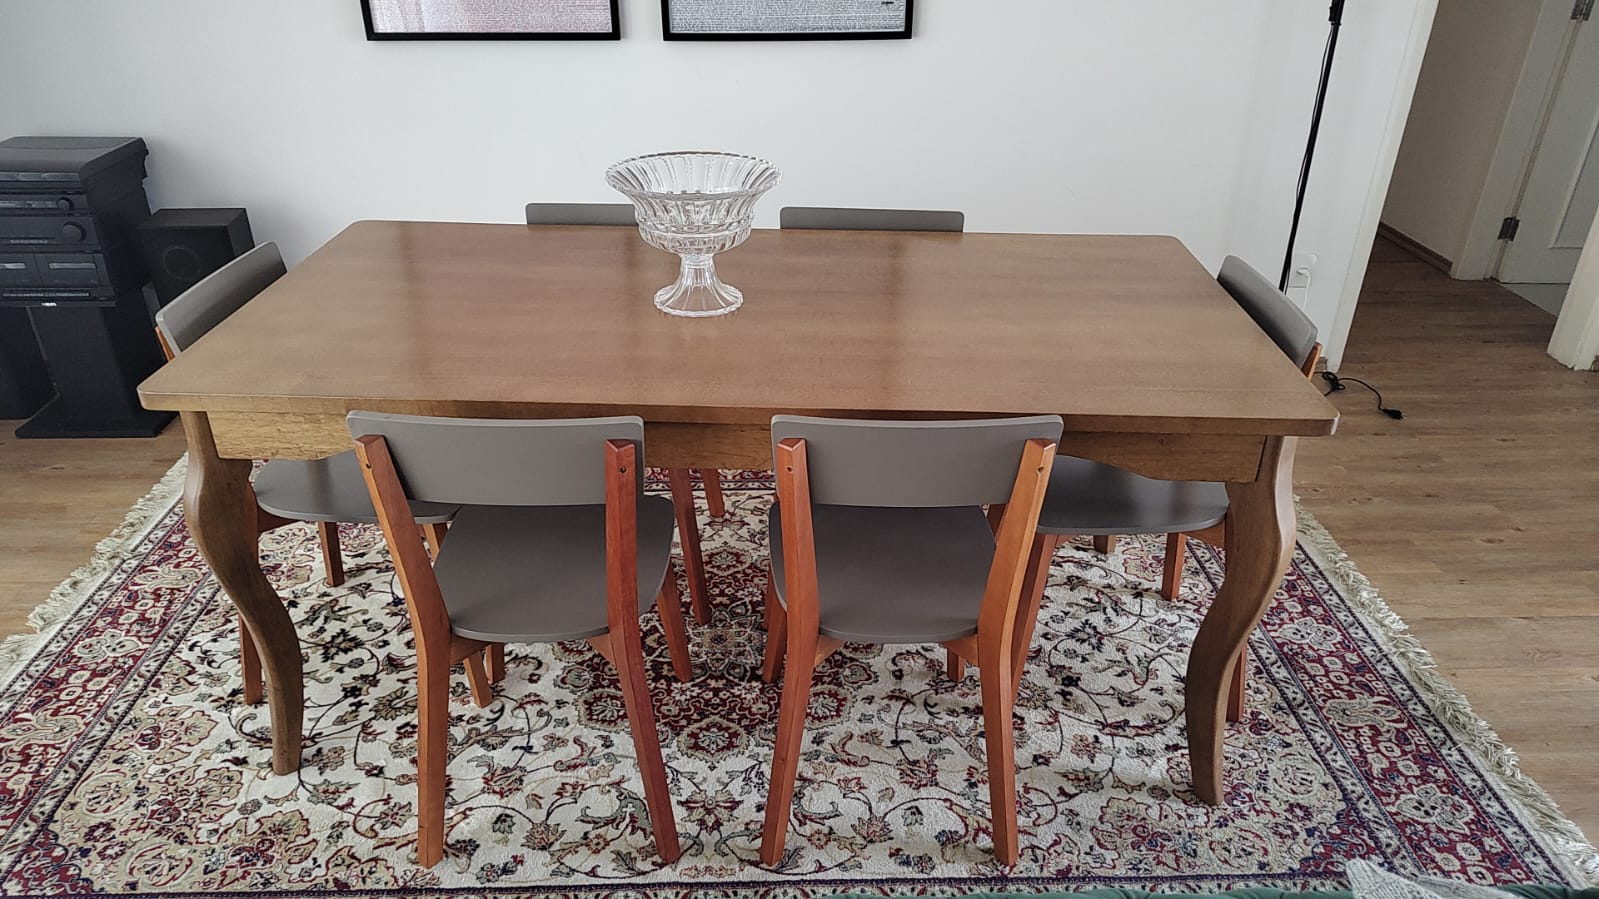
\includegraphics[width=\textwidth]{./MEDIA/MESA_JANTAR.jpeg}
\caption{Mesa de jantar Luís XV com seis cadeiras.}
\end{figure}

\textbf{Medidas}
\begin{itemize}
\item Largura: 180 cm (em torno de)
\item Altura: 100 cm (em torno de)
\end{itemize}

\textbf{Valor}
\begin{itemize}
\item 1.900 reais
\end{itemize}
                    
\endgroup
\vfill
\pagebreak       % [Frontistício]
%%\newcommand{\linhalayout}[2]{{\tiny\textbf{#1}\quad#2\par}}
\newcommand{\linha}[2]{\ifdef{#2}{\linhalayout{#1}{#2}}{}}

\begingroup\tiny
\parindent=0cm
\thispagestyle{empty}

\textbf{edição brasileira©}\quad			 {Hedra \the\year}\\
\textbf{organização©}\quad		 			 {Acácio Augusto}\\
\textbf{tradução e notas©}\quad		 		 {Mariana Lins}\\
\textbf{apresentação©}\quad			 		 {Acácio Augusto e Helena Wilke}\\
%\textbf{tradução©}\quad			 		 {Mariana Lins}\\
%\textbf{ilustração©}\quad			 		 {copyrightilustracao}\medskip

%\textbf{título original}\quad			 	 {}\\
%\textbf{edição consultada}\quad			 {edicaoconsultada}\\
%\textbf{primeira edição}\quad			 	 {Acontecimentos}\\
%\textbf{agradecimentos}\quad			 	 {Acácio Augusto}\\
%\textbf{indicação}\quad			 		 {indicacao}\medskip

\textbf{edição}\quad			 			 {Jorge Sallum}\\
\textbf{coedição}\quad			 			 {Suzana Salama}\\
\textbf{editor assistente}\quad			 	 {Paulo Henrique Pompermaier}\\
\textbf{revisão e preparação}\quad			 {Rogério Duarte}\\
%\textbf{preparação}\quad			 		 {Rogério Duarte}\\
%\textbf{iconografia}\quad			 		 {iconografia}\\
\textbf{capa}\quad			 				 {Lucas Kröeff}\\
%\textbf{imagem da capa}\quad			 	 {imagemcapa}\medskip

\textbf{\textsc{isbn}}\quad			 		 {978-85-7715-726-6}

\hspace{-5pt}\begin{tabular}{ll}
\textbf{conselho editorial} & Adriano Scatolin,  \\
							& Antonio Valverde,  \\
							& Caio Gagliardi,    \\
							& Jorge Sallum,      \\
							& Ricardo Valle,     \\
							& Tales Ab'Saber,    \\
							& Tâmis Parron      
\end{tabular}
 
\vfill
 
\begin{minipage}{8cm}
\textbf{Dados Internacionais de Catalogação na Publicação (CIP)\\
(Câmara Brasileira do Livro: \textsc{sp}, Brasil)}

\textbf{\hrule}\smallskip

Cleyre, Voltairine de, 1866--1912\\

\textit{Ação direta e outros escritos}. Voltairine de
Cleyre; organização Acácio Augusto; tradução e notas Mariana Lins. 1ª\,ed. São Paulo, \textsc{sp}: Editora Hedra, 2023.\\

\textsc{isbn} 978-85-7715-726-6\\

1. Anarquismo 2. Anarquistas: Livros e leitura 3. Antologia 4. Filosofia\\ 
\textsc{i}. Augusto, Acácio. \textsc{ii}. Lins, Mariana. \textsc{iii}. Título.\\

23--170052 \hfill \textsc{cdd}: 320.57

\textbf{\hrule}\smallskip

\textbf{Elaborado por Eliane de Freitas Leite (CRB--8/\,8415)}\\

\textbf{Índices para catálogo sistemático:}\\
1. Anarquismo: Ciência política (320.57)
\end{minipage}

\vfill

\textit{Grafia atualizada segundo o Acordo Ortográfico da Língua\\
Portuguesa de 1990, em vigor no Brasil desde 2009.}\\

\textit{Direitos reservados em língua\\
portuguesa somente para o Brasil}\\\medskip

\textsc{editora hedra ltda.}\\
Av.~São Luís, 187, Piso 3, Loja 8 (Galeria Metrópole)\\
01046--912 São Paulo \textsc{sp} Brasil\\
Telefone/Fax +55 11 3097 8304\\\smallskip
editora@hedra.com.br\\
www.hedra.com.br\\

\bigskip

Foi feito o depósito legal.

\endgroup
\pagebreak     % [Créditos]
%% Tamanhos
% \tiny
% \scriptsize
% \footnotesize
% \small 
% \normalsize
% \large 
% \Large 
% \LARGE 
% \huge
% \Huge

% Posicionamento
% \centering 
% \raggedright
% \raggedleft
% \vfill 
% \hfill 
% \vspace{Xcm}   % Colocar * caso esteja no começo de uma página. Ex: \vspace*{...}
% \hspace{Xcm}

% Estilo de página
% \thispagestyle{<<nosso>>}
% \thispagestyle{empty}
% \thispagestyle{plain}  (só número, sem cabeço)
% https://www.overleaf.com/learn/latex/Headers_and_footers

% Compilador que permite usar fonte de sistema: xelatex, lualatex
% Compilador que não permite usar fonte de sistema: latex, pdflatex

% Definindo fontes
% \setmainfont{Times New Roman}  % Todo o texto
% \newfontfamily\avenir{Avenir}  % Contexto

\begingroup\thispagestyle{empty}\vspace*{.05\textheight} 

              \formular
              \LARGE
              \noindent
              \textsc{Ação direta e\\outros escritos}
              % \smallskip
                      
              % \large
              % \noindent\textit{}
              % \normalsize 
              \bigskip  
              
              \Large
              \noindent
              \textbf{Voltairine de Cleyre}
              
              \vspace{3.5em}

              \newfontfamily\minion{Minion Pro}
              \fontsize{30}{40}\selectfont \minion\small

              \noindent Acácio Augusto (\textit{organização})

              \noindent Mariana Lins (\textit{tradução e notas})

              \noindent Emma Goldman (\textit{posfácio})\\

              \vspace{3.5em}
              
              \noindent
              {\fontsize{30}{40}\selectfont \minion\small\noindent 1ª edição}

              \vfill

              \newfontfamily\timesnewroman{Times New Roman}
              {\noindent\fontsize{30}{40}\selectfont \timesnewroman hedra}
              \smallskip
              
              {\selectfont\minion\small
              \noindent São Paulo \quad\the\year}

\endgroup
\pagebreak
	       % [folha de rosto]
% nothing			is level -3
% \book				is level -2
% \part				is level -1
% \chapter 			is level 0
% \section 			is level 1
% \subsection 		is level 2
% \subsubsection 	is level 3
% \paragraph 		is level 4
% \subparagraph 	is level 5
\setcounter{secnumdepth}{-2}
\setcounter{tocdepth}{0}

% \renewcommand{\contentsname}{Índex} 	% Trocar nome do sumário para 'Índex'
%\ifodd\thepage\relax\else\blankpage\fi 	% Verifica se página é par e coloca página branca
%\tableofcontents*

% \pagebreak
% \begingroup \footnotesize \parindent0pt \parskip 5pt \thispagestyle{empty} \vspace*{-0.5\textheight}\mbox{} \vfill
% \baselineskip=.92\baselineskip
% \input{PRETAS.tex}
% \endgroup

% \pagebreak
% {\begingroup\mbox{}\pagestyle{empty}
% \pagestyle{empty} 
% % \renewcommand{\contentsname}{Índex} 	% Trocar nome do sumário para 'Índex'
% \addtocontents{toc}{\protect\thispagestyle{empty}}
% \movetooddpage
% \tableofcontents*\clearpage\endgroup}

%\input{Y-publicidade}	   % [lista de livros publicados]
%\pagebreak

\ifodd\thepage\blankpage\fi

\parindent=0pt
\footnotesize\thispagestyle{empty}

% \noindent\textbf{Dados Internacionais de Catalogação na Publicação -- CIP}\\
% \noindent\textbf{(Câmara Brasileira do Livro, SP, Brasil)}\\

% \dotfill\\

% \hspace{20pt}ISBN 978-65-86238-31-0 (Livro do Estudante)

% \hspace{20pt}ISBN 978-65-86238-30-3 (Manual do Professor)\\[6pt]

% \hspace{20pt}\parbox{190pt}{1. Crônicas Brasileira. 2. Contos Brasileiro. 3. Rosa, Alexandre. I. Título.}\\[6pt]

% \hspace{188pt}\textsc{cdd}-B869.8

% \dotfill

% \noindent{}Elaborado por Regina Célia Paiva da Silva CRB -- 1051\\

\mbox{}\vfill
\begin{center}
		\begin{minipage}{.7\textwidth}\tiny\noindent{}
		\centering\tiny
		Adverte-se aos curiosos que se imprimiu este 
		livro na gráfica Meta Brasil, 
		na data de \today, em papel pólen soft, composto em tipologia Minion Pro e Formular, 
		com diversos sofwares livres, 
		dentre eles Lua\LaTeX e git.\\ 
		\ifdef{\RevisionInfo{}}{\par(v.\,\RevisionInfo)}{}\medskip\\\
		\adforn{64}
		\end{minipage}
\end{center}		   % [colofon]


